\clearpage%
\setcounter{page}{6}
\twocolumn

\begin{table*}[b!]
    \centering
    \caption*{\raggedright \hspace{1.3em} \textbf{Таблица}}
    \begin{tabular}{|c|c|c|c|c|c|c|c|c|c|c|c|c|c|c|c|c|}
    \hline
    0 & 1 & 2 & 3  & 4  & 5 & 6  & 7  & 8  & 9  & 10 & 11 & 12 & 13 & 14 & 15 & 16 \\ \hline
    1 & 3 & 9 & 10 & 13 & 5 & 15 & 11 & 16 & 14 & 8  & 7  & 4  & 12 & 2  & 6  & 1  \\ \hline
    \end{tabular}
\end{table*}
уравнений: сначала решается уравнение (4), корнями которого яявляются суммы $\epsilon_1 + \epsilon_4$ и $\epsilon_2 + \epsilon_3$ симметричных (см. рис. 6!) корней уравнения (3), а затем из уравнений (5) находятся и сами корни уравнения (3).
Именно таким путем Гауссу удалось осуществить построение правильного 17-угольника: здесь тоже выделяются группы корней, суммы которых находятся последовательно из квадратных уравнений. Но как искать эти "хорошие" группы? Гаусс находит удивительный путь ответить на этот вопрос...

\section{\label{sec:intro}Построение правильного 17-угольника}
\begin{small}
{\textbf{
30 марта 1796 наступает для Гаусса день творческого крещения... Гаусс уже занимался с некоторого времени группировкой корней из единицы на основании своей теории "первообразных" корней. И вот однажды утром, проснувшись, он внезапно ясно и отчетливо осознал, что из его теории вытекает построение семнадцатиугольника... Это событие явилось поворотным пунктом жизни Гаусса. Он принимает решения посвятить себя не филологии, и исключительно математике.}}
\end{small}\\
(\textit{Ф.Клейн})

Чтобы выявить найденные Гауссом скрытые "симметрии" в множестве корней 17-й степени из единицы и разбить корни на нужные группы, введем новую нумерацию корней. Будем возводить 3 в последовательной степени 0, 1, 2,... и каждый раз брать остаток от деления полученного числа на 17. Избавимся от проведения этих выкладок и в таблице приведем окончательные результаты. В первой строке стоят показатели k, а под ними остатки от деления $3^{k}$ на 17. \\
\begin{figure}[t]
    %\centering
    \setcounter{figure}{6}
    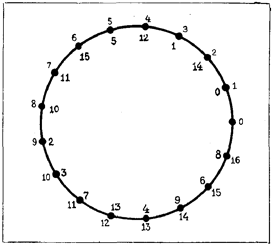
\includegraphics[width = \columnwidth]{2.png}
    \label{fig:17_angle}
    \caption{Старые номера корней даны черным цветом, новые - красным.}
\end{figure}
Обратите внимание, что в нижней строке содержатся все числа от 1 до 16; затем $3^{16}$ дает остаток 1 и далее остатки периодически повторяются (докажите!).

Закономерность, подмеченная Гауссом, является частным случаем следующе теоремы: \textbf{для всякого простого p существует такое число l, называемое первообразным корнем, что среди остатков от деления $l^k$ на p встречаются все числа 1, 2, ..., p - 1}. Этот факт впервые отметил Эйлер (1707-1783), но смог доказать лишь Лежандр (1752-1833); другое доказательство получил Гаусс, но, вероятно, в 1796 году он еще не обладал общей теоремой, а обнаружил приведенный факт эмпирически, проводя вычисления для конкретных чисел. Это очень важное обстоятельство, не учитывая которого, трудно правильно понять природу ранних работ Гаусса.
Присвоем корну $\epsilon_k$, $k=3^l$, новый номер, а именно l, который мы

\clearpage

\section{\label{sec:intro}Правильные n-угольники и корни из единицы}

Преобразуем уравнение $z^n - 1$:
$$z^n - 1 \;=\;(z - 1) \times (z^{n-1} + z^{n-2} + ... + z + 1)\;=\;0.$$

Получим два уравнения: $z = 1$ и $z^{n-1} + z^{n-2} + ... + z + 1\;=\;0.$ (2)

Уравнение (2) имеет своими корнями $\epsilon_k$ при $1 \leq k \leq n - 1.$ В дальнейшем мы будем иметь дело с уравнением (2).

При $n = 3$ получаем уравнение $z^2 + z + 1 = 0.$ Его корни: $\epsilon_1 \;=\; - \dfrac{1}{2} + i\dfrac{\sqrt{3}}{2}$ и $\epsilon_2 \;=\; - \dfrac{1}{2} - i\dfrac{\sqrt{3}}{2}$ (рис.5.)
\setcounter{page}{2}
\begin{figure}[h!]
    \centering
    \setcounter{figure}{4}
    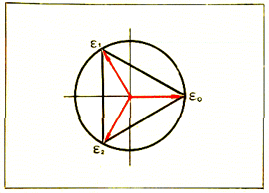
\includegraphics[scale=0.7]{1.png}
    \label{fig:3_angle}
    \caption{     }
\end{figure}
